\documentclass[a4paper,12pt]{extarticle} \usepackage[utf8]{inputenc}
\usepackage[T1]{fontenc}
\usepackage[margin=2.5cm]{geometry}

% Fonte Caladea se existir, senão lmodern
\IfFileExists{caladea.sty}{
  \usepackage{caladea}
}{
  \usepackage{lmodern} }
\usepackage{ragged2e}
\usepackage{graphicx}
\usepackage{hyperref}
\usepackage{fancyhdr}
\usepackage{xcolor}
\usepackage{rotating}
\usepackage{titlesec}
\usepackage{dirtytalk}
\usepackage[portuguese]{babel}
\usepackage{indentfirst} % Indenta o primeiro parágrafo após seções
\usepackage{epigraph} % Indenta o primeiro parágrafo após seções


% Ajuste do recuo de parágrafo
\setlength{\parindent}{1.5em}

% Centralizar títulos
\titleformat{\section}
  {\normalfont\centering\bfseries\Large}{\thesection}{1em}{}

\titleformat{\subsection}
  {\normalfont\centering\bfseries\large}{\thesubsection}{1em}{}

\titleformat{\subsubsection}
  {\normalfont\centering\bfseries}{\thesubsubsection}{1em}{}

% -------------- Símbolos de Versículo e Resposta --------------
% Definição do símbolo (a “barrinha” inclinada)
\makeatletter
\newcommand{\vers@resp@sym}{%
  \raisebox{0.2ex}{\rotatebox[origin=c]{-20}{$\m@th\rceil$}}%
}
% macro interna que sobrepõe a barrinha e a letra V ou R
\newcommand{\vers@resp}[2]{%
  {\ooalign{%
     \hidewidth\kern#1\vers@resp@sym\hidewidth\cr
     #2\cr
  }}%
}
% comandos públicos \versicle e \response
\DeclareRobustCommand{\versicle}{\vers@resp{-0.1em}{V}}
\DeclareRobustCommand{\response}{\vers@resp{0pt}{R}}
\makeatother
% ^------------- Símbolos de Versículo e Resposta -------------^

% Rodapé com imagem e página
\pagestyle{fancy}
% ---- Cabeçalho ------------
\fancyhf[C]{}
% ----- Rodapé --------------
\fancyfoot[LO,LE]{%
  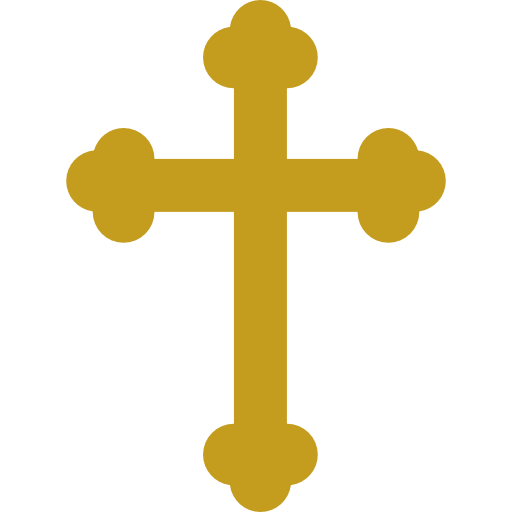
\includegraphics[scale=0.2]{assets/cross.png}\quad
  \textit{São Sisto II, rogai por nós.}
}
\fancyfoot[RO,RE]{\thepage}

\begin{document}

\begin{center}
  \textbf{\LARGE Novena a São Sisto II e seus Companheiros Mártires}\\[0.5em]
  \say{ Naquele tempo, Jesus disse aos discípulos: “Se alguém quer me seguir, renuncie a si mesmo, tome a sua cruz e me siga. Pois quem quiser salvar a sua vida vai perdê-la; e quem perder a sua vida por causa de mim, vai encontrá-la.
De fato, de que adianta ao homem ganhar o mundo inteiro mas perder a sua vida? Que poderá alguém dar em troca de sua vida? Porque o Filho do Homem virá na glória do seu Pai, com os seus anjos, e então retribuirá a cada um de acordo com a sua conduta. Em verdade vos digo: Alguns daqueles que estão aqui não morrerão antes de verem o Filho do Homem vindo com o seu Reino”. }\\
  \epigraph{
    -- (Mt 16, 24-28)
  }

\end{center}

\tableofcontents
\thispagestyle{empty}

% --- Vida / Origem da Novena ---
\newpage

\section{História}

\subsection{Contexto histórico}

Os anos que se seguiram de 250 até 260 foram uns dos mais terríveis e, ao mesmo tempo, gloriosos do Cristianismo: terríveis, devido à fúria dos imperadores Décio e Valeriano; e gloriosos, por conta da têmpera dos inúmeros mártires que foram os que mais glorificaram a Deus.

\subsection{Papado}

O Santo Papa Sisto II, a quem celebramos neste dia, foi um desses homens que soube transformar o terrível em glória, a partir do seu testemunho de fé, amor e esperança em Cristo Jesus. Pertence à lista de cinco consecutivos Papas mártires, São Sisto II governou a Igreja durante um ano (257 – 258) e, nesse tempo, semeou a paz e a unidade no seio da Igreja de Cristo.

\subsection{Mártires}

Foi decapitado pela polícia durante uma cerimônia clandestina que ele celebrava num cemitério da via Ápia. Foram, ao mesmo tempo, executados seis dos sete diáconos que o rodeavam. Só pouparam algum tempo o diácono Lourenço, seu tesoureiro, a quem deixaram quatro dias para entregar os bens da Igreja. Assim se procedia desde que o imperador Valeriano (+260) estabelecera a pena de morte “sem julgamento, só com verificação de identidade”, contra os Bispos, padres e diáconos da religião cristã.

\subsection{Testemunho}

Dessa forma, São Sisto II e seus companheiros mártires entregaram a vida deles em sinal de fidelidade a Cristo e foram recompensados com o tesouro da eternidade no Céu. O martírio torna-se um grande testemunho para a comunidade cristã, além de fomentar a fé na vida eterna e na verdade do Evangelho. A comunidade a qual esses homens participavam foi enriquecida e amadurecida pela dor da tragédia transformada em alegria e admiração popular.


\newpage
\section{Orações}

\subsection{Oração Inicial} \label{oracao-inicial}

\textbf{Em nome do Pai, do Filho e do Espírito Santo. Amém.}

Ó São Sisto II, que fostes elevado ao sólio pontifício num século em que a Igreja ainda sofria as violências e perseguições do Império Romano, e que fostes capturado e decapitado, morrendo mártir por amor a Nosso Senhor,  
ensinai-nos a amar e a escolher sempre o caminho do bem.  
E, se for para a maior glória de Nosso Senhor, intercedei por nós pelas graças que vos pedimos nesta novena.  \textbf{Amém.}

\begin{center}
  \large
  \textbf{Pai-Nosso, Ave-Maria e Glória.}
\end{center}


\subsection{Oração Final} \label{oracao-final}

Pai Todo-Poderoso, que concedestes a São Sisto II e seus companheiros a graça de dar a vida por causa da Vossa Palavra e do testemunho de Jesus,  
pela força do Espírito Santo, fazei-nos dóceis para acolher a fé e fortes para proclamá-la.  
Por Nosso Senhor Jesus Cristo, Vosso Filho, que convosco vive e reina na unidade do Espírito Santo,  
por todos os séculos dos séculos.  





\vfill

\begin{center}
\subsection*{Fontes:}
\href{https://santo.cancaonova.com/santo/sao-sisto-ii-papa-e-seus-companheiros-diaconos/}{Canção Nova}\\ 
\href{https://www.youtube.com/watch?v=sgsIK4bPKgE&list=PLRL6i6PPLb5-3ktc9DIPs50VmSLCTu0ok}{Canal Virtude Plena}
\end{center}


\end{document}
